%% AMS-LaTeX Created with the Wolfram Language : www.wolfram.com

\documentclass{article}
\usepackage{amsmath, amssymb, graphics, setspace}

\newcommand{\mathsym}[1]{{}}
\newcommand{\unicode}[1]{{}}

\newcounter{mathematicapage}
\begin{document}

\begin{doublespace}
\noindent\(\pmb{\text{Clear}[\text{{``}Global$\grave{ }$*{''}}];}\\
\pmb{a\text{:=}2;}\\
\pmb{\text{Remove}[\text{ffund},\text{orthDeriv}];}\\
\pmb{\text{ffund}\text{:=}\text{Log}[(\#\#[[1]]{}^{\wedge}2+\#\#[[2]]{}^{\wedge}2){}^{\wedge}(1/2)]\&;}\\
\pmb{\text{orthDeriv}[\text{f$\_$},\text{xy$\_$}]\text{:=}\{-D[f[\{x,y\}],y],D[f[\{x,y\}],x]\}\text{/.}\, \{x\to \text{xy}[[1]],y\to \text{xy}[[2]]\};}\\
\pmb{\text{e1}\text{:=}\{1,0\};}\\
\pmb{\text{f1}\text{:=}\text{ffund}[\#\#-\text{e1}]+\text{ffund}[\#\#+\text{e1}]\&;}\\
\pmb{\text{g1}\text{:=}\text{orthDeriv}[\text{f1},\#\#] \&;}\\
\pmb{\text{Remove}[x,y];}\)
\end{doublespace}

\begin{doublespace}
\noindent\(\pmb{\text{StreamPlot}\left[\text{g1}[\{x,y\}],\{x,-a,a\},\{y,-a,a\}, \text{StreamPoints}\text{-$>$}\text{Fine},\text{FrameLabel}\text{-$>$}\left\{x_1,x_2\right\},
\text{RegionFunction}\text{-$>$}\text{Function}[\{x,y,\text{vx},\text{vy},n\},-1<\text{f1}[\{x,y\}]<1]\right]}\)
\end{doublespace}

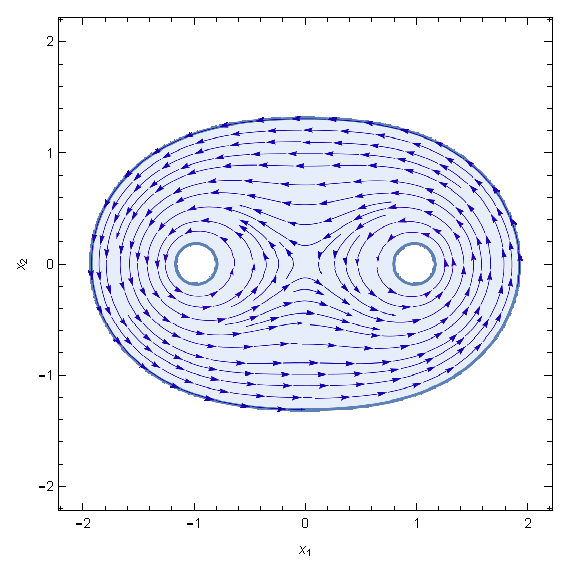
\includegraphics{HarmonicVectorFields_gr1.eps}

\begin{doublespace}
\noindent\(\pmb{\text{f2}\text{:=}\text{ffund}[\#\#-\text{e1}]-\text{ffund}[\#\#+\text{e1}]+\#\#[[1]]\&;}\\
\pmb{\text{g2}\text{:=}\text{orthDeriv}[\text{f2},\#\#] \&}\\
\pmb{\text{StreamPlot}\left[\text{g2}[\{x,y\}],\{x,-a,a\},\{y,-a,a\},\text{StreamPoints}\text{-$>$}\text{Fine},\text{FrameLabel}\text{-$>$}\left\{x_1,x_2\right\},\text{RegionFunction}\text{-$>$}\text{Function}[\{x,y,\text{vx},\text{vy},n\},-0.7<\text{f2}[\{x,y\}]<0.7
\&\& -2<y<2]\right]}\)
\end{doublespace}

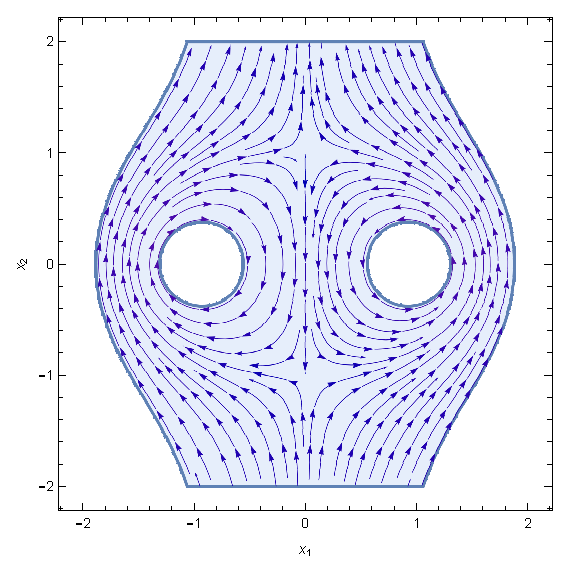
\includegraphics{HarmonicVectorFields_gr2.eps}

\begin{doublespace}
\noindent\(\pmb{\text{f3}\text{:=}\text{ffund}[\#\#-\text{e1}]+\#\#[[1]]\&;}\\
\pmb{\text{g3}\text{:=}\text{orthDeriv}[\text{f3},\#\#] \&}\\
\pmb{\text{StreamPlot}\left[\text{g3}[\{x,y\}],\{x,-a,a\},\{y,-a,a\},\text{StreamPoints}\text{-$>$}\text{Fine},\text{FrameLabel}\text{-$>$}\left\{x_1,x_2\right\},\text{RegionFunction}\text{-$>$}\text{Function}[\{x,y,\text{vx},\text{vy},n\},-0.5<\text{f3}[\{x,y\}]<2
\&\& -2<y<2]\right]}\)
\end{doublespace}

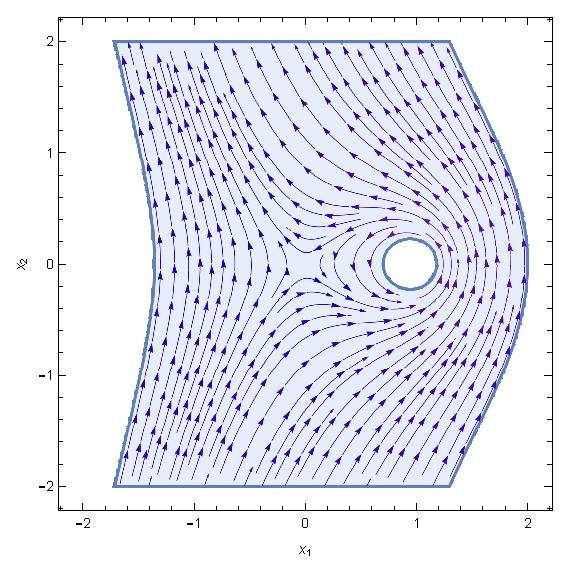
\includegraphics{HarmonicVectorFields_gr3.eps}

\begin{doublespace}
\noindent\(\pmb{\text{Animate}\left[\text{StreamPlot}\left[(1-\text{lambda})*\text{g1}[\{x,y\}]+\text{lambda}*\text{g2}[\{x,y\}],\{x,-a,a\},\{y,-a,a\},\text{FrameLabel}\text{-$>$}\left\{x_1,x_2\right\},
\text{StreamPoints}\text{-$>$}\text{Fine}\right],\{\text{lambda},0,1\},\text{AnimationRunning}\text{-$>$}\text{False}, \right.}\\
\pmb{\text{AnimationRate}\to .05]}\)
\end{doublespace}

\begin{doublespace}
\noindent\(\fbox{$
\begin{array}{l}
  \\
  \\
\end{array}
$}\)
\end{doublespace}

\begin{doublespace}
\noindent\(\pmb{\text{Animate}\left[\text{VectorPlot}\left[(1-\text{lambda})*\text{g1}[\{x,y\}]4+\text{lambda}*\text{g2}[\{x,y\}],\{x,-a,a\},\{y,-a,a\},\text{FrameLabel}\text{-$>$}\left\{x_1,x_2\right\},
\text{VectorPoints}\text{-$>$}\text{Fine}\right],\{\text{lambda},0,1\},\text{AnimationRunning}\text{-$>$}\text{False}, \right.}\\
\pmb{\text{AnimationRate}\to .05]}\)
\end{doublespace}

\begin{doublespace}
\noindent\(\fbox{$
\begin{array}{l}
  \\
  \\
\end{array}
$}\)
\end{doublespace}

\begin{doublespace}
\noindent\(\pmb{\text{regionOmega}=\text{RegionDifference}[\text{Disk}[\{0,0\},4],\text{RegionUnion}[\text{Disk}[\{-2,0\},1],\text{Disk}[\{2,0\},1]]];}\\
\pmb{\text{solveDirichlet}[\text{uBoundary$\_$}]\text{:=}\text{Module}[\{\text{uval}\},}\\
\pmb{\text{LaplaceEquation2D}=\{\text{Laplacian}[u[x,y],\{x,y\}]\text{==}0, \text{DirichletCondition}[u[x,y]\text{==}\text{uBoundary}[x,y],\text{True}]\};}\\
\pmb{\text{(*}\text{Dsolve}[\text{LaplaceEquation2D}, u[x,y],x,y]\text{*)}}\\
\pmb{\text{uval}=\text{NDSolveValue}[\text{LaplaceEquation2D},u,\{x,y\}\in \text{regionOmega}][\#\#[[1]],\#\#[[2]]]\&;\text{uval}]}\\
\pmb{\text{uBoundary}=\text{If}[\text{$\#$1}{}^{\wedge}2+\text{$\#$2}{}^{\wedge}2>15,0,1]\&;}\\
\pmb{\text{f4} = \text{solveDirichlet}[\text{uBoundary}];}\\
\pmb{\text{g4}\text{:=}\text{orthDeriv}[\text{f4},\#\#]\&;}\)
\end{doublespace}

\begin{doublespace}
\noindent\(\pmb{\text{StreamPlot}\left[\text{Evaluate}[\text{g4}[\{x,y\}]],\{x,y\}\in \text{regionOmega},\text{FrameLabel}\text{-$>$}\left\{x_1,x_2\right\},
\text{StreamPoints}\text{-$>$}\text{Fine}\right]}\)
\end{doublespace}

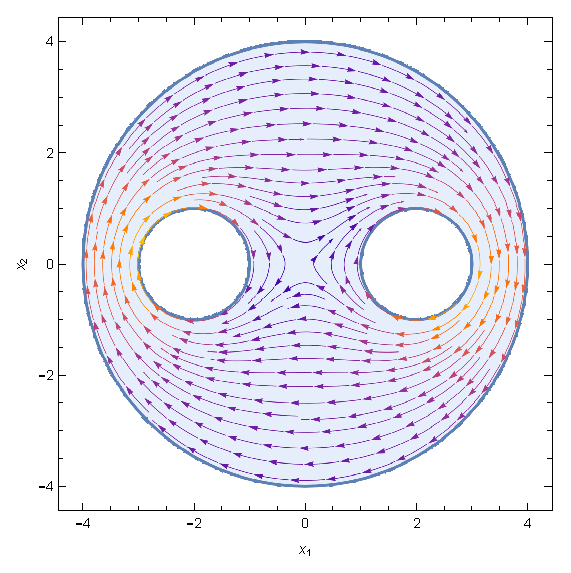
\includegraphics{HarmonicVectorFields_gr4.eps}

\begin{doublespace}
\noindent\(\pmb{\text{}}\\
\pmb{\text{uBoundary}=\text{If}[\text{$\#$1}{}^{\wedge}2+\text{$\#$2}{}^{\wedge}2>15,0,\text{If}[\text{$\#$1}>0,-1,1]]\&;}\\
\pmb{\text{f5} = \text{solveDirichlet}[\text{uBoundary}];}\\
\pmb{\text{g5}\text{:=}\text{orthDeriv}[\text{f5},\#\#]\&;}\\
\pmb{\text{StreamPlot}\left[\text{Evaluate}[\text{g5}[\{x,y\}]],\{x,y\}\in \text{regionOmega},\text{FrameLabel}\text{-$>$}\left\{x_1,x_2\right\},
\text{StreamPoints}\text{-$>$}\text{Fine}\right]}\)
\end{doublespace}

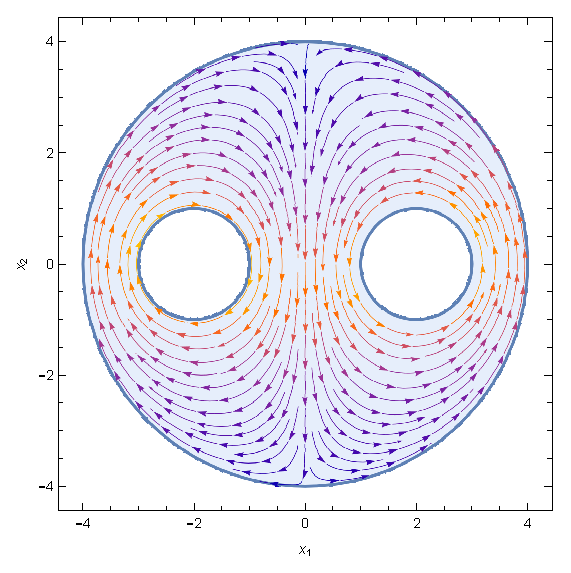
\includegraphics{HarmonicVectorFields_gr5.eps}

\begin{doublespace}
\noindent\(\pmb{\text{Animate}\left[\text{StreamPlot}\left[\text{Evaluate}[(1-\text{lambda})*\text{g4}[\{x,y\}]+\text{lambda}*\text{g5}[\{x,y\}]],\{x,y\}\in
\text{regionOmega},\text{FrameLabel}\text{-$>$}\left\{x_1,x_2\right\}, \text{StreamPoints}\text{-$>$}\text{Fine}\right],\{\text{lambda},0,1\},\right.}\\
\pmb{\text{AnimationRunning}\text{-$>$}\text{False}, \text{AnimationRate}\to .05]}\)
\end{doublespace}

\begin{doublespace}
\noindent\(\fbox{$
\begin{array}{l}
  \\
  \\
\end{array}
$}\)
\end{doublespace}

\end{document}
